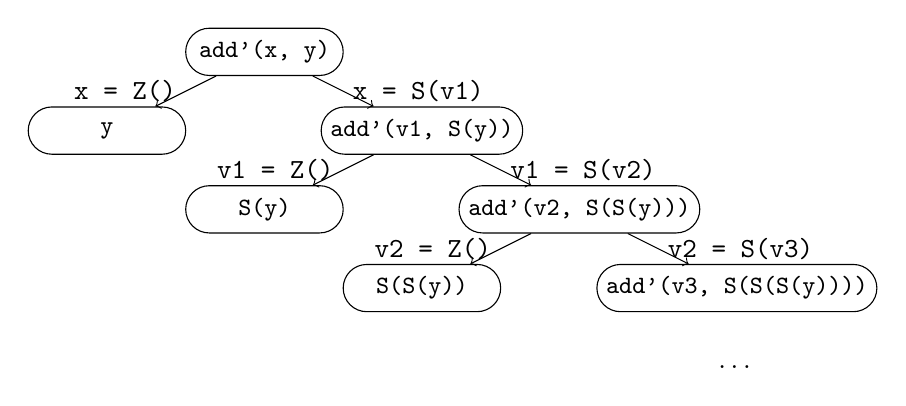
\begin{tikzpicture}[
level distance=10mm,
level/.style={sibling distance=40mm},
conf/.style={
	rectangle,minimum width=20mm,minimum height=6mm,rounded corners=3mm,
	draw=black,
	font=\ttfamily\small} 
]
\node[conf] {add'(x, y)} 
	child[->] {
		node[conf] {y}
		edge from parent node[left] {\texttt{x = Z()}}
	}
	child[->] {
		node[conf] {add'(v1, S(y))} 
		child[->] {
			node[conf] {S(y)}
			edge from parent node[left] {\texttt{v1 = Z()}}
		}
		child[->] {
			node[conf] {add'(v2, S(S(y)))} 
			child[->] {
				node[conf] {S(S(y))}
				edge from parent node[left] {\texttt{v2 = Z()}}
			}
			child[->] {
				node[conf] {add'(v3, S(S(S(y))))}
				child {node {\ldots} edge from parent[draw=none]}
				edge from parent node[right] {\texttt{v2 = S(v3)}}
			}
			edge from parent node[right] {\texttt{v1 = S(v2)}}
		}
		edge from parent node[right] {\texttt{x = S(v1)}}
	};
		
\end{tikzpicture}